\chapter{Introduction}
\label{cha:intro}
The first contains a general introduction to the work. The goals are
defined and the modus operandi is explained.
\todo{bib referenties in orde brengen}
\section{Introduction}

Security is an important asset in Computer Science. Defending a network of a company is not an easy job. To prevent intruders it can make use of firewalls, routers, IDS systems, virus scans, and other defence mechanisms. Unfortunately technology is growing fast and attacks are getting more sophisticated and the causes of these attacks can be very different. \todo{iets tussen nog} Companies are often the victim of targeted attacks. In a security report of 2014, \todo{verwijzing naar report}, states that 80\% of the companies are the victims of targeted attacks. Many companies don't see themselves as a target, but sometimes they might be collateral, the target on the way to the real target. This means that everybody can be a target. 
Corporate networks should continuously defend themselves against outside invaders such as viruses and worms. By doing so the network administrator can keep the network as malware-free as possible. If there is  an intruder managed to penetrate the network then the network manager this intruder trying to get out as quickly as possible. This is not always easy. Especially when the intruders secretly sneak and then spread rapidly.
In this paper we will work further on the work made by Marten van Dijk, Ari Juels, Alina Oprea and Ronals L. Rivest \todo{verwijzing naar FlipIT} who wrote a report on the Game FlipIt. FlipIt is a the game of '' Stealthy Takeovers''. It models a game by means of two players, the attacker and the defender. Both can gain control over a single shared resource by flipping it. The most important property of the game is that the flipping happens stealthy. This means that the players have no clue about when the other player moves. The goal of the game is to maximise the time the player controls the resource minus the average cost of the flipping. 

\subsection{Motivation of the game}
%waarom FlipIt gebruiken en niet iets anders.
\subsection{Contributions and results}
\subsection{Conclusions}


\section{introduction number 2}

(We live in an era) In this era where digitalization becomes prominent in every aspect of our lives, where technology is growing fast and where business are always under attack, security becomes an issue of increasing complexity. Since 2009, the number of reported security attacks on companies has increased 66\%, year over year. \todo{security report van pwc}. These numbers only represent the attacks that are detected. In 2014 117,339 attacks where coming in daily. Many of those attacks have a different cause. Some of them can be benign, others can be harmful. Many companies are unaware of all the attacks. Some of them think that they are not a target, but they might be a target on the way to a real target. Recently there where some high profiled targeted attacks which have been revealed. (Belgacom). 
Targeted attacks are ...
The \textit{Kill Chain} is a concept by Lockheed Martin Corporation, explained in the whitepaper \todo{withepaper toevoegen}. It explains the different phases of a typical attack from the view of an attacker. It also outlines the typical attacker activities on the right. This model is very useful to define the different moments of the life cycle of an attack and when a company should act to defend itself. In this paper we would like to prevent the viruses of spreading into the network system of a company. This means that we have to act in phase Installation, Command and Control and Action on Objectives of the kill chain. 

 
  Security is an important asset in Computer Science. Defending a network of a company is not an easy job. Malicious people will try to  To prevent intruders it can make use of firewalls, routers, IDS systems, virus scans, and other defence mechanisms. Unfortunately technology is growing fast and attacks are getting more sophisticated and the causes of these attacks can be very different. \todo{iets tussen nog} Companies are often the victim of targeted attacks. In a security report of 2014, \todo{verwijzing naar report}, states that 80\% of the companies are the victims of targeted attacks. Many companies don't see themselves as a target, but sometimes they might be collateral, the target on the way to the real target. This means that everybody can be a target. 
Corporate networks should continuously defend themselves against outside invaders and targeted attacks. Researchers have already investigated the situations through the FlipIt game in which a system is continuously compromised by an attacker through targeted attacks. 
FlipIt is a the game of '' Stealthy Takeovers''. It models a game by means of two players, the attacker and the defender. Both can gain control over a single shared resource by flipping it. The most important property of the game is that the flipping happens stealthy. This means that the players have no clue about when the other player moves and has control over the shared resource. The goal of the game is to maximise the time the player controls the resource minus the average cost of the number of flipping.
In this paper we model a company network through multiple shared resources and a flip from the attacker that drops a virus that will spread itself autonomously. We show that ...

\section{Virusses}

Stealth
Regin's developers put considerable effort into making it highly inconspicuous. Its low key nature means it can potentially be used in espionage campaigns lasting several years. Even when its presence is detected, it is very difficult to ascertain what it is doing. Symantec was only able to analyze the payloads after it decrypted sample files.

It has several ''stealth'' features. These include anti-forensics capabilities, a custom-built encrypted virtual file system (EVFS), and alternative encryption in the form of a variant of RC5, which isn't commonly used. Regin uses multiple sophisticated means to covertly communicate with the attacker including via ICMP/ping, embedding commands in HTTP cookies, and custom TCP and UDP protocols
%http://www.symantec.com/connect/blogs/regin-top-tier-espionage-tool-enables-stealthy-surveillance
Ways of defending a network:
\begin{itemize}
\item Self-defending networks: The next generation of network security
\item Honeynet games: a game theoretic approach to defending network monitors

\end{itemize}
Many network security threats today are spread over the Internet. The most common include:

Viruses, worms, and Trojan horses
Spyware and adware
Zero-day attacks, also called zero-hour attacks
Hacker attacks
Denial of service attacks
Data interception and theft
Identity theft

%http://www.ists.dartmouth.edu/library/258.pdf Email Virus Propagation Modeling and Analysis
%Cliff C. Zou∗, Don Towsley†, Weibo Gong∗
%∗Department of Electrical & Computer Engineering
%†Department of Computer Science
%Univ. Massachusetts, Amherst
%Technical Report: TR-CSE-03-04

Computer virus through mail. 
Though virus spreading through email is an old technique, it is still effective and is widely used by
current viruses and worms. Sending viruses through email has some advantages that are attractive to
virus writers:
 Sending viruses through email does not require any security holes in computer operating systems
or software.
 Almost everyone who uses computers uses email service.
 A large number of users have little knowledge of email viruses and trust most email they receive,
especially email from their friends [28][29].
 Email are private properties like post office letters. Thus correspondent laws or policies are required
to permit checking email content for detecting viruses before end users receive email [18].

Send a email with malicious attachment. Only again infected if attachment again opened. Thus this is the action of attacking every neighbour node + also can attack again the node where the virus was coming from.
There are also email viruses were the malicious program is hidden in the txt and the attachment does not need to be opened. 


Spy vs Spy: Aldrich Ames was a CIA Counter-Intelligence officer. He was also a spy feeding valuable intelligence to the Soviets and compromising US intelligence operations in the Soviet Union. He operated for 9 years before the CIA recognized that they had a spy and began an investigation and determined that he was the leak. This strategic situation is the same one faced by computer networks, drug cartels, intelligence agencies and guerrilla networks.

All such organisations have a reasonable expectation that trusted personal/systems will eventually be recruited/captured by enemy organisations. Therefore such organisations must consume valuable resources to discover such betrayals and thereby regain secrecy. The question is then given the possible threats how often and at what cost should they spend resources on investigations/spy hunts/virus scans. This is where flipIt comes in.

FLIPIT: The Game of ''Stealthy Takeover:'' FlipIt was created to model these sorts of strategic situations and to study the best courses of action. Specifically flipIt was motivated by the recent interest in and success of Advanced Persistent Threats, or APT.

The basic idea is that given the current experience that perfect protection of trusted resources is unattainable, lets think about how we can optimally manage compromises of the our most trusted systems.

Rules

Two players, player X (blue) and player Y (red) attempt to maintain control over a shared resource.
At anytime in the game each player is allowed to play 'flip'.
The only way a player can learn the state of the game (who is in control) is when they play flip.
If a player is in control of the resource and they play flip they remain in control of the resource.
If a player is not in control of the resource and they play flip they gain control of the resource.
Players gain points for the length of time they control the resource.
Players lose points every time they play flip.
This reflects the situation that the CIA is placed in with regard to moles/enemy spies. They don't know if they have been compromised. They can perform an investigation and determine if they have been compromised, also catching the spy in the act, but this action is very expensive. That is, the CIA has to trade off between remaining''mole free'' (a good) and investigations (an expense).

Winning: How do you win a fair game of flipIt against intelligent adaptive human adversaries? I'm not sure.

In the real world what is the best move given that the other players can secretly capture/corrupt your most trusted personal/systems? Rives suggests in his talk that you:
Be prepared to deal with repeated total failure (loss of control).
Play fast! Aim to make opponent drop out!
Arrange game so that your moves cost much less than your opponent's!
%http://www.cisco.com/web/offer/gist_ty2_asset/Cisco_2014_ASR.pdf p49
%http://repo.hackerzvoice.net/depot_madchat/vxdevl/papers/avers/2004-35.pdf
%http://www.mcafee.com/us/resources/white-papers/foundstone/wp-managing-malware-outbreak.pdf



\subsection{Malware}
%Does a company network faces lot of malware? what is the cost ?
Relevant researches:
\begin{itemize}
%http://ants.iis.sinica.edu.tw/3BkMJ9lTeWXTSrrvNoKNFDxRm3zFwRR/17/04483668.pdf
\item How Viruses and worm can be detected. Difference between UDP en TCP worm propagation
\end{itemize}




%%%%%%%%%%%%%%%%%%%%%%%%%%%%%%%%%%%%%%%%%%%%%%%%%%%%%%%%%%
%%%%%			Conclusion Chapter 1				%%%%%%
%%%%%												%%%%%%
%%%%%												%%%%%%
%%%%%%%%%%%%%%%%%%%%%%%%%%%%%%%%%%%%%%%%%%%%%%%%%%%%%%%%%%
\section{Conclusion}
\label{Cha:1:Conclusion}
The final section of the chapter gives an overview of the important results
of this chapter. This implies that the introductory chapter and the
concluding chapter don't need a conclusion.


%%% Local Variables: 
%%% mode: latex
%%% TeX-master: "thesis"
%%% End: 

%\end{document}

%\begin{minipage}{0.5\textwidth}
%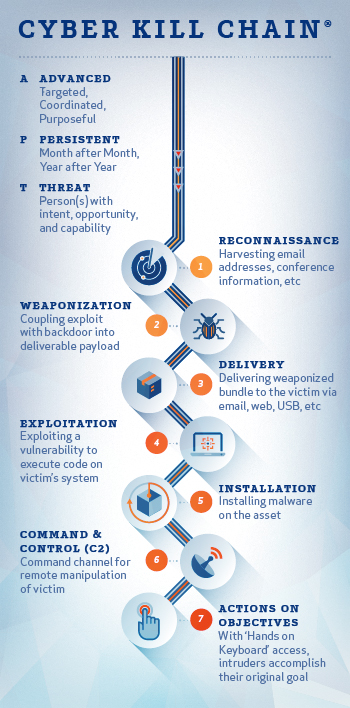
\includegraphics{Images/killchain.jpg}
%\end{minipage} \hfill
%\begin{minipage}{0.45\textwidth}
%\begin{itemize}
%\item *Rectangle
%\item *Color: blue
%\end{itemize}
%\end{minipage}

%http://www.pwc.com/gx/en/consulting-services/information-security-survey/index.jhtml
%%% Local Variables: 
%%% mode: latex
%%% TeX-master: "thesis"
%%% End: 
